\chapter{Cluster Ridgelines Plots}
\label{ape:joyplots}


In this appendix all the distributions from the aggregated characteristics of each cluster are summarized using ridgeline plots, with the exception of the \code{constant\_ratio}, because only one cluster has datasets with constant features.

Each cluster is represented by a different color, with the number of the cluster displayed in the y axis. The x axis is the value of the variable, and the height of each distribution is the frequency, like in a histogram.

\singlespacing

\renewcommand{\arraystretch}{0.85}
\captionsetup{margin=1.0cm}  % correção nas margens dos captions.


\begin{figure}[!ht]
    \centering
    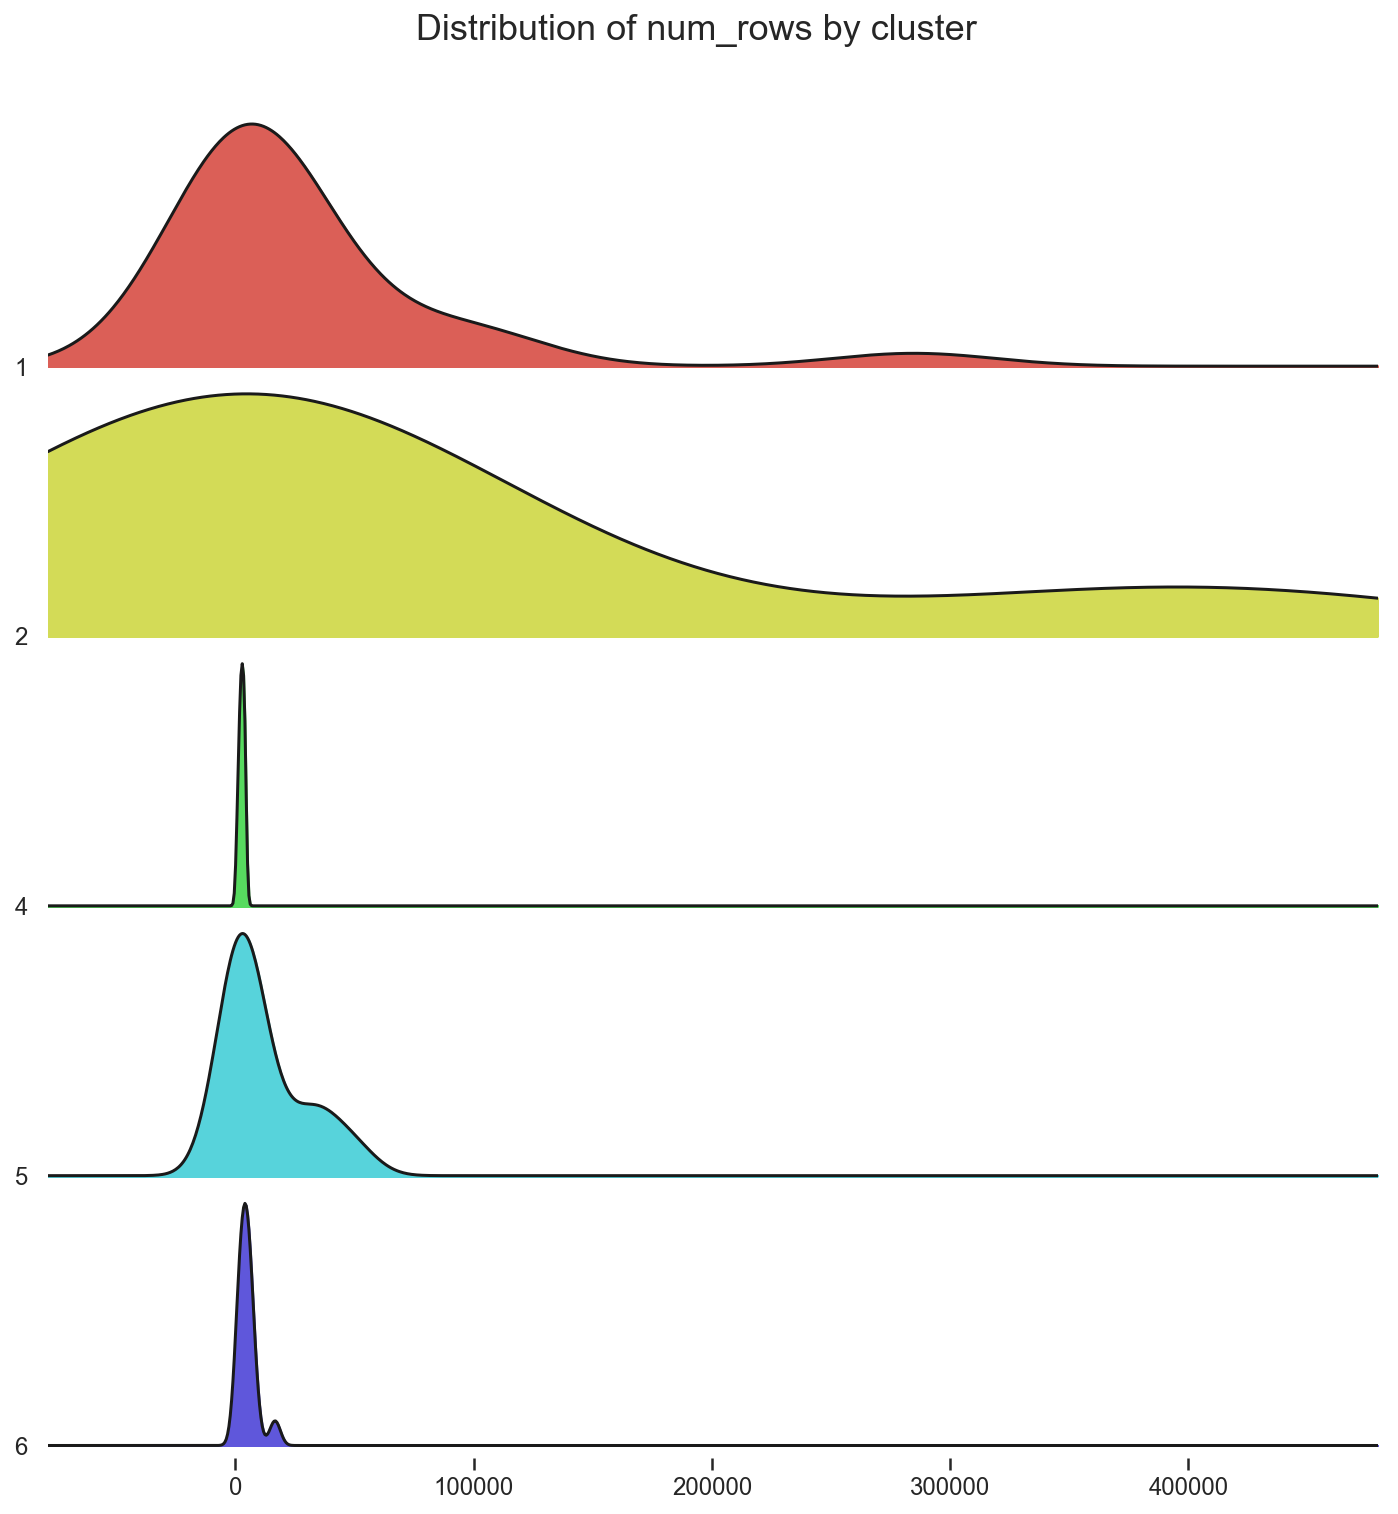
\includegraphics[width=.7\textwidth, height=.7\textwidth]{appendix_figures/joyplot_1.png}
    \caption{Ridgeline plot of \code{num\_rows} }
\end{figure}
\begin{figure}[!ht]
    \centering
    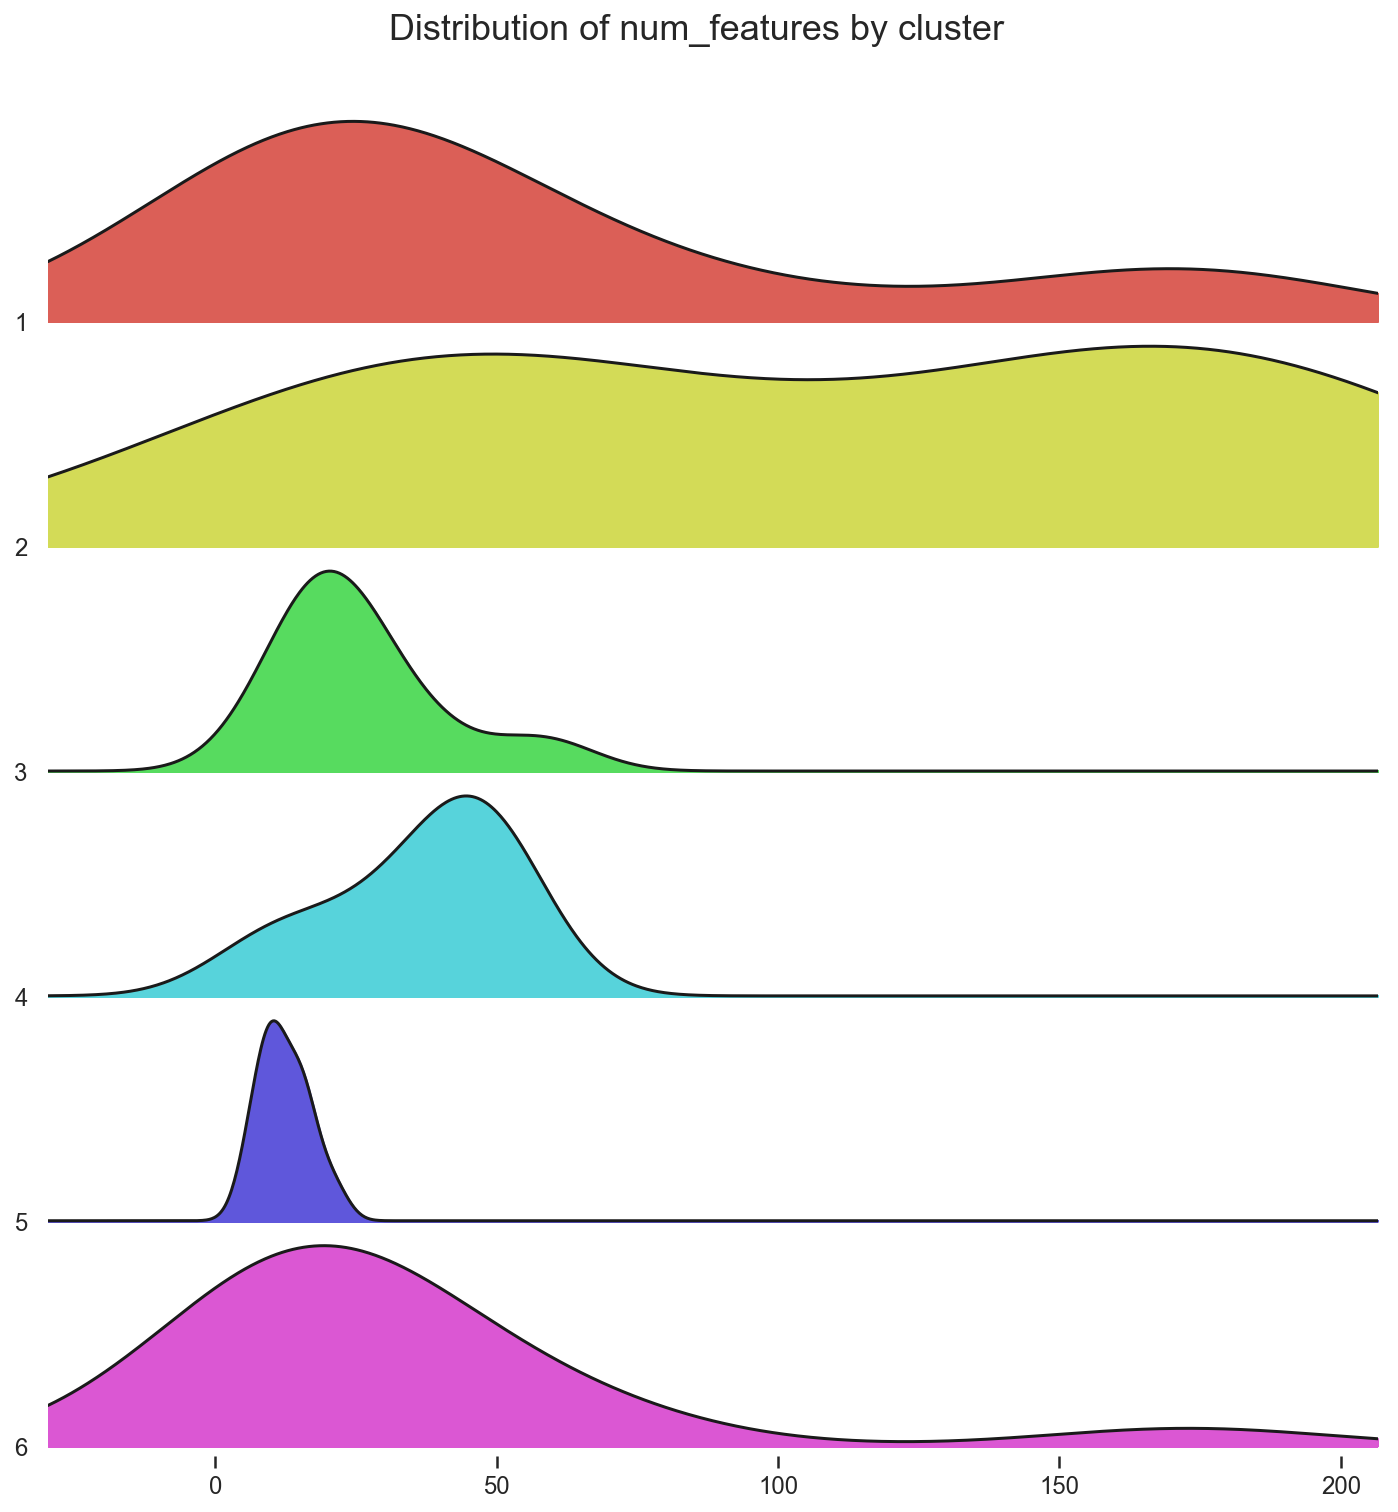
\includegraphics[width=.7\textwidth, height=.7\textwidth]{appendix_figures/joyplot_2.png}
    \caption{Ridgeline plot of \code{num\_features} }
\end{figure}
\begin{figure}[!ht]
    \centering
    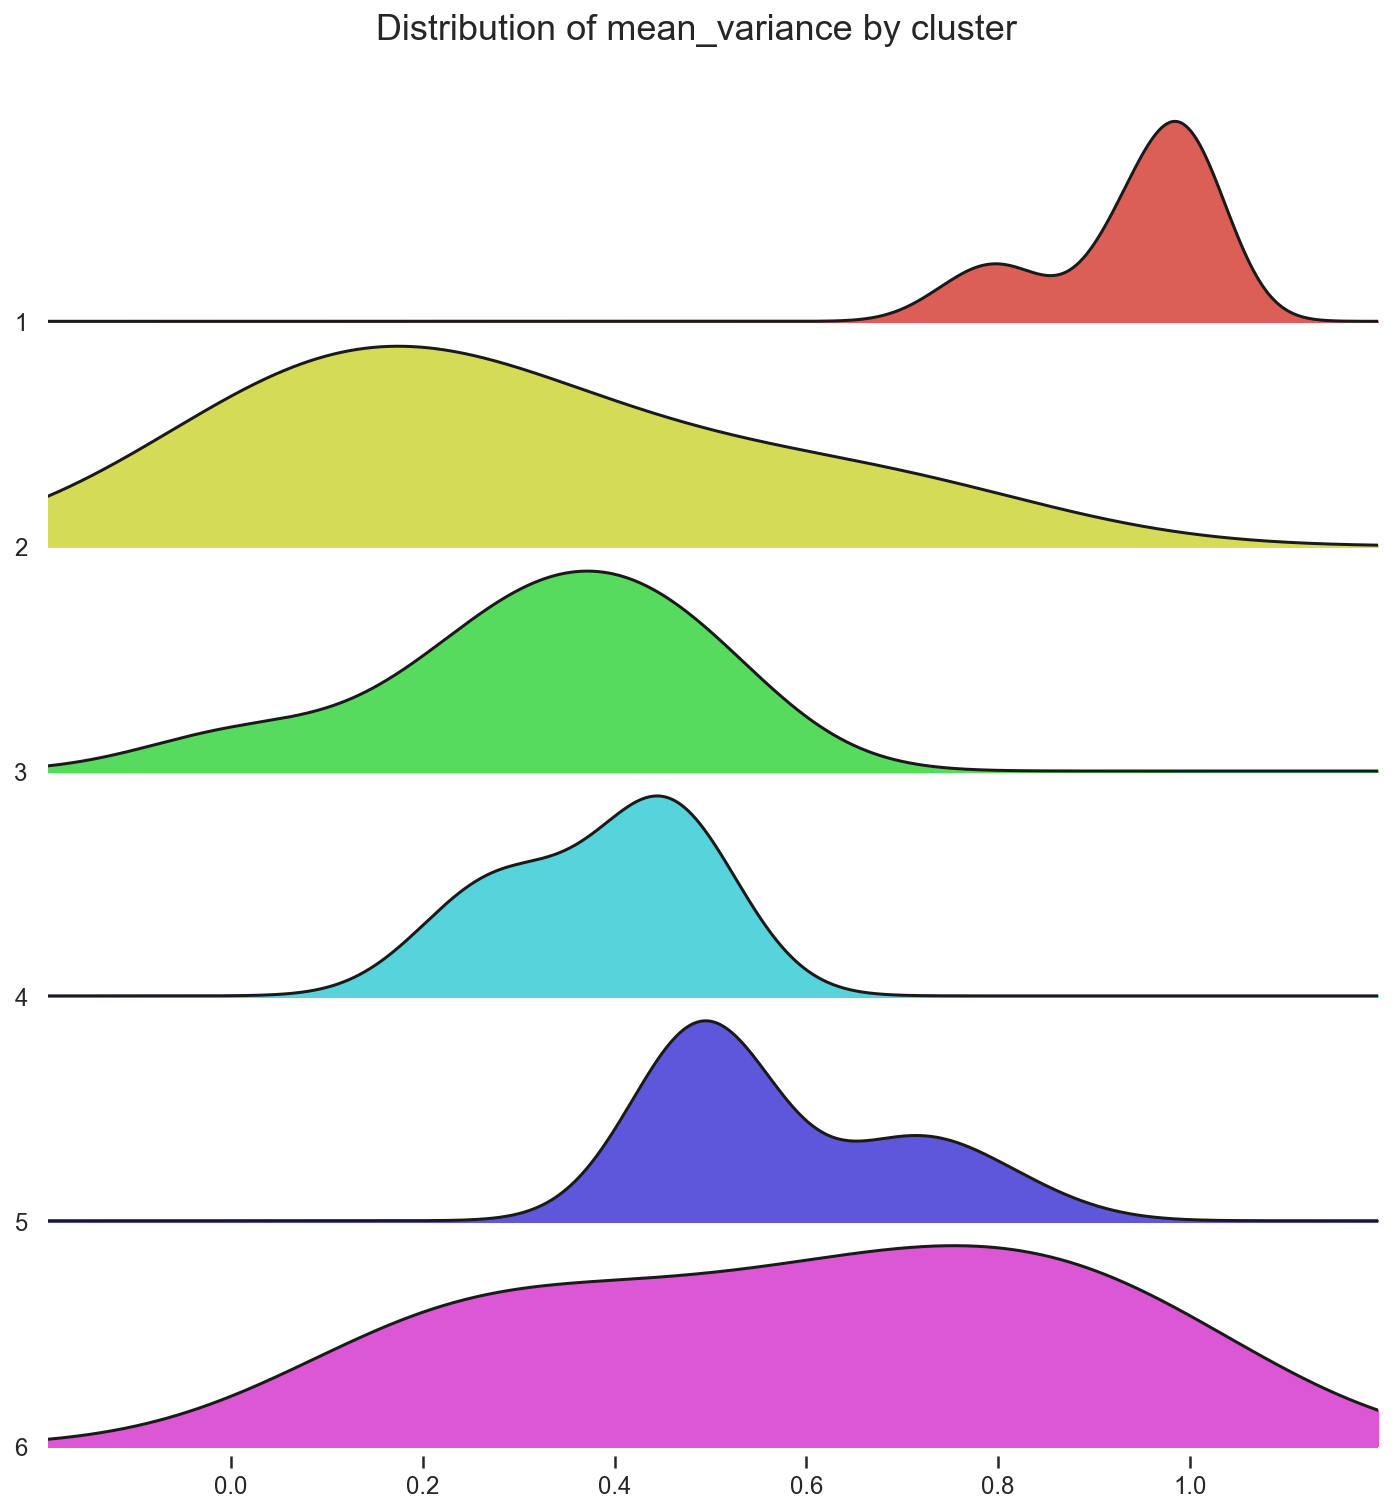
\includegraphics[width=.7\textwidth, height=.7\textwidth]{appendix_figures/joyplot_3.png}
    \caption{Ridgeline plot of \code{mean\_variance} }
\end{figure}
\begin{figure}[!ht]
    \centering
    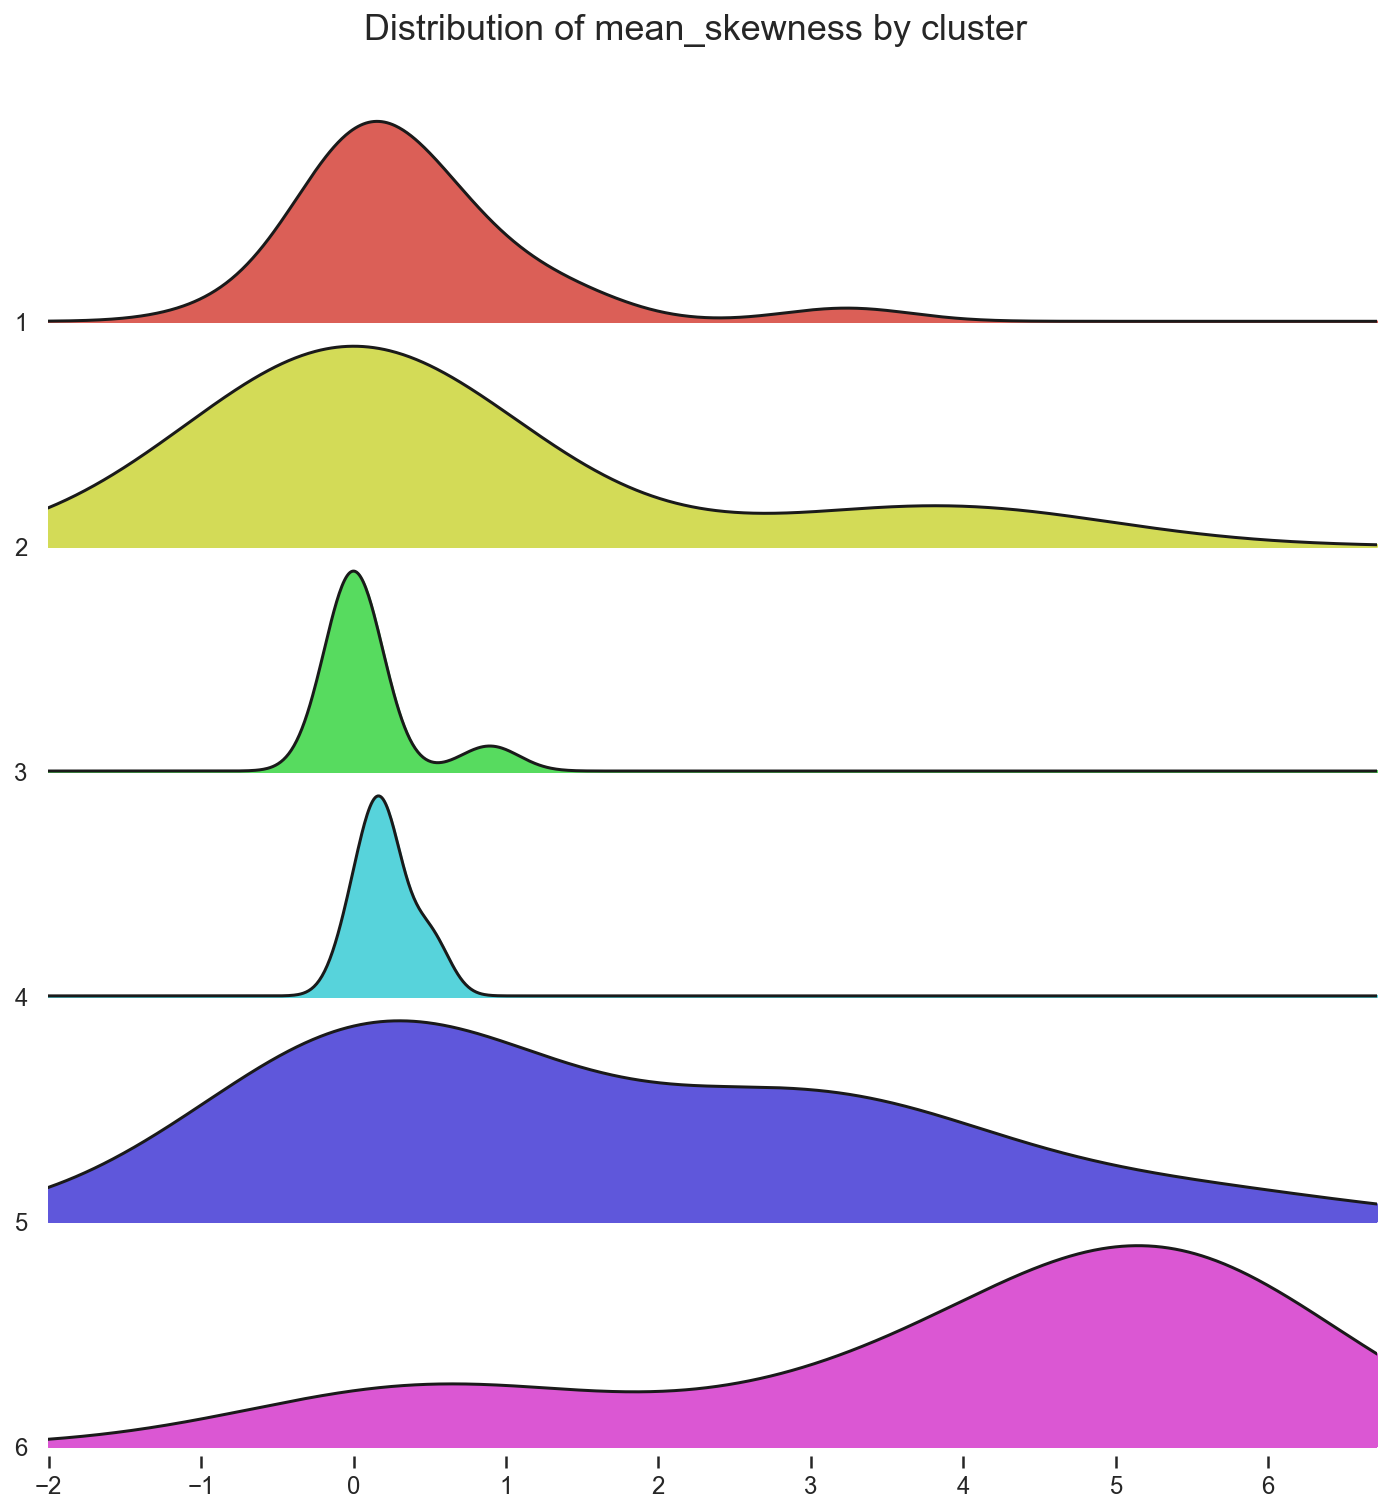
\includegraphics[width=.7\textwidth, height=.7\textwidth]{appendix_figures/joyplot_4.png}
    \caption{Ridgeline plot of \code{mean\_skewness} }
\end{figure}
\begin{figure}[!ht]
    \centering
    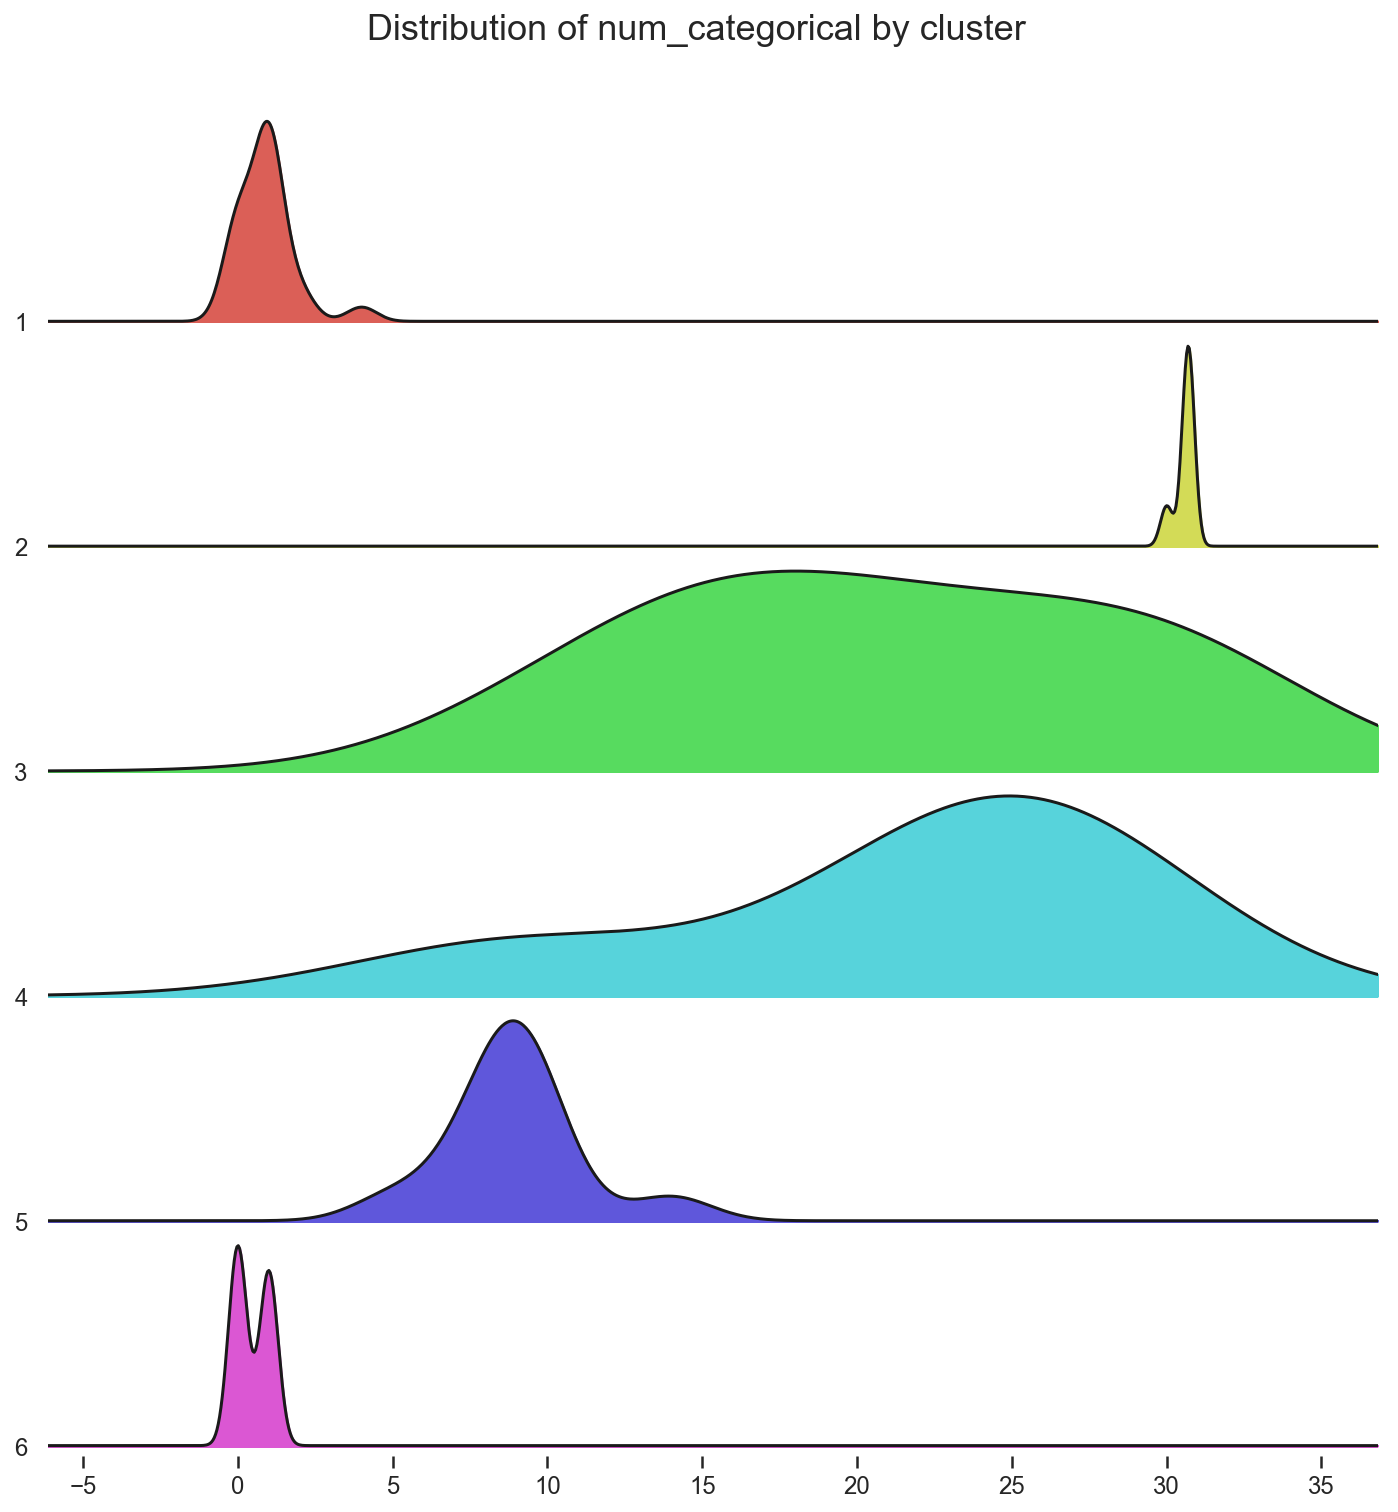
\includegraphics[width=.7\textwidth, height=.7\textwidth]{appendix_figures/joyplot_5.png}
    \caption{Ridgeline plot of \code{num\_categorical} }
\end{figure}
\begin{figure}[!ht]
    \centering
    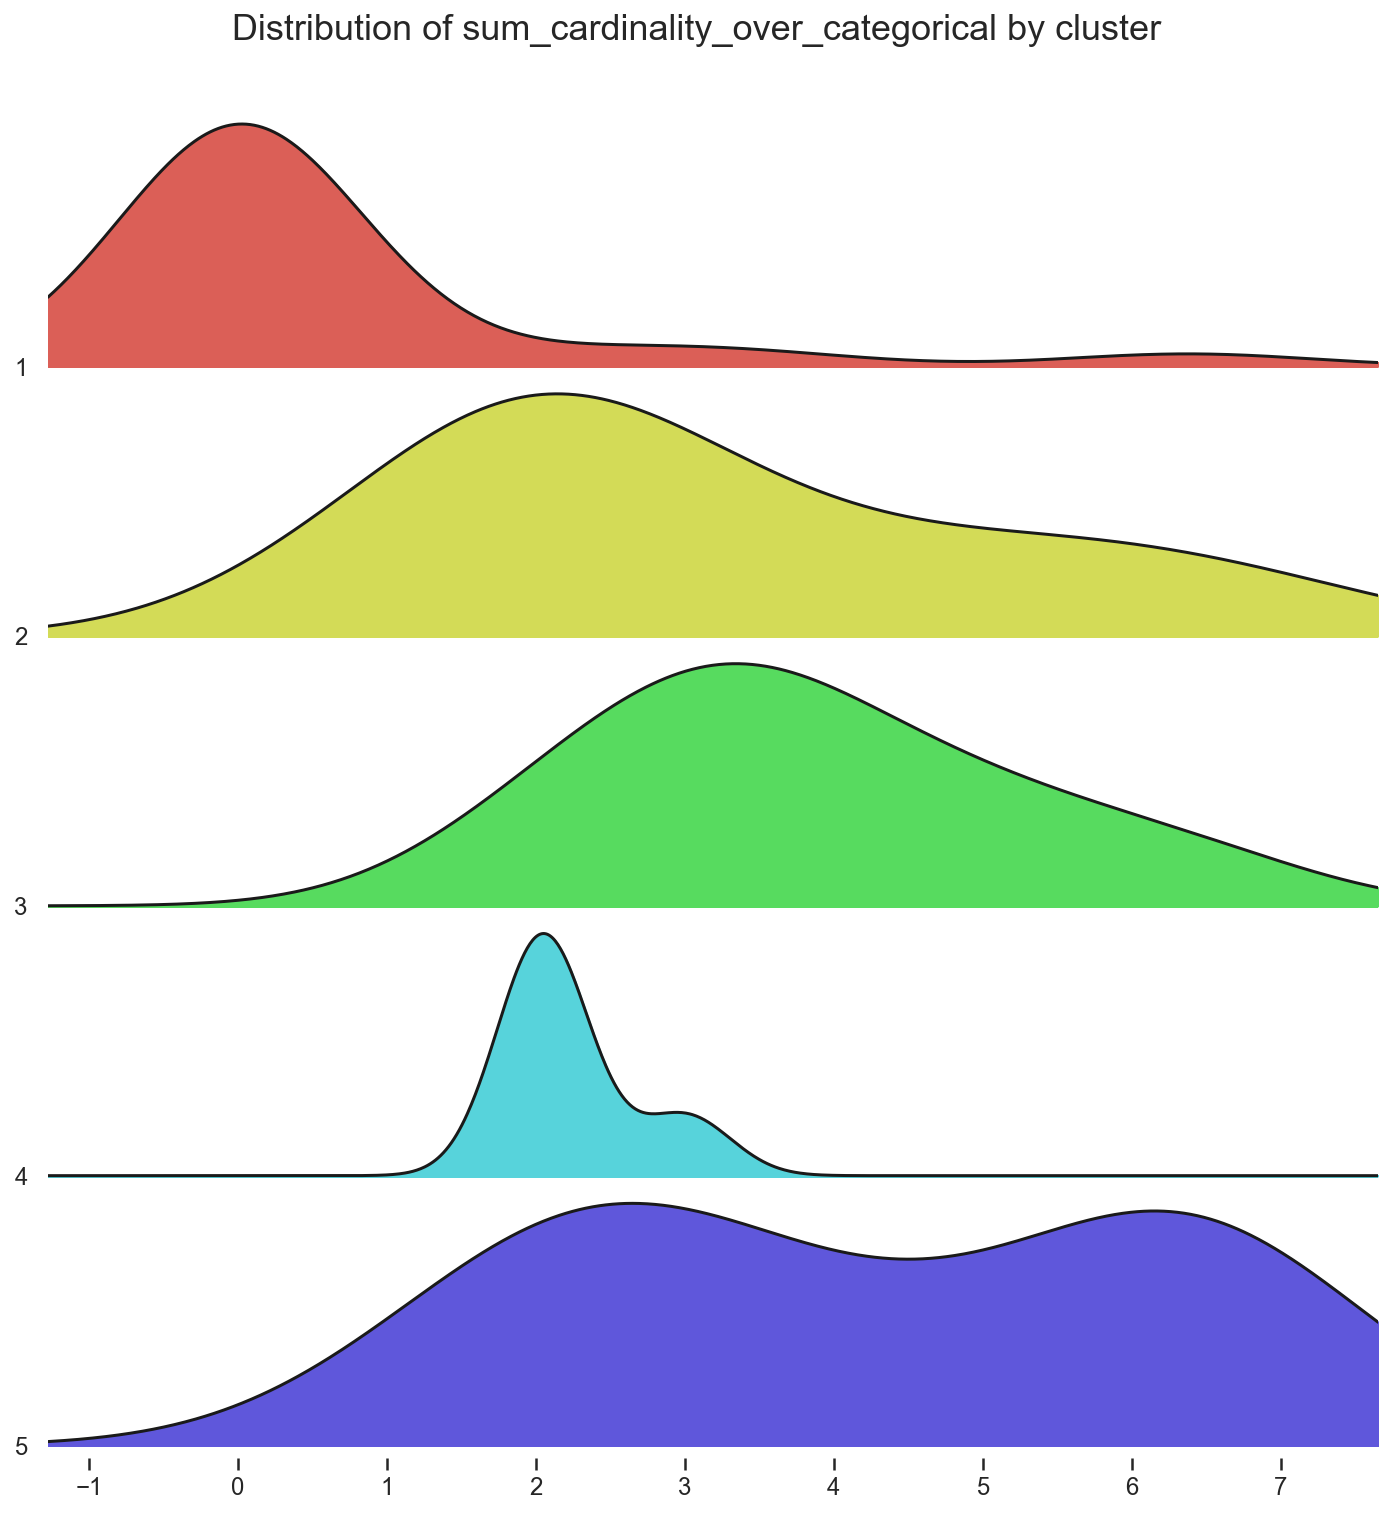
\includegraphics[width=.7\textwidth, height=.7\textwidth]{appendix_figures/joyplot_6.png}
    \caption{Ridgeline plot of \code{sum\_cardinality\_over\_categorical} }
\end{figure}
\begin{figure}[!ht]
    \centering
    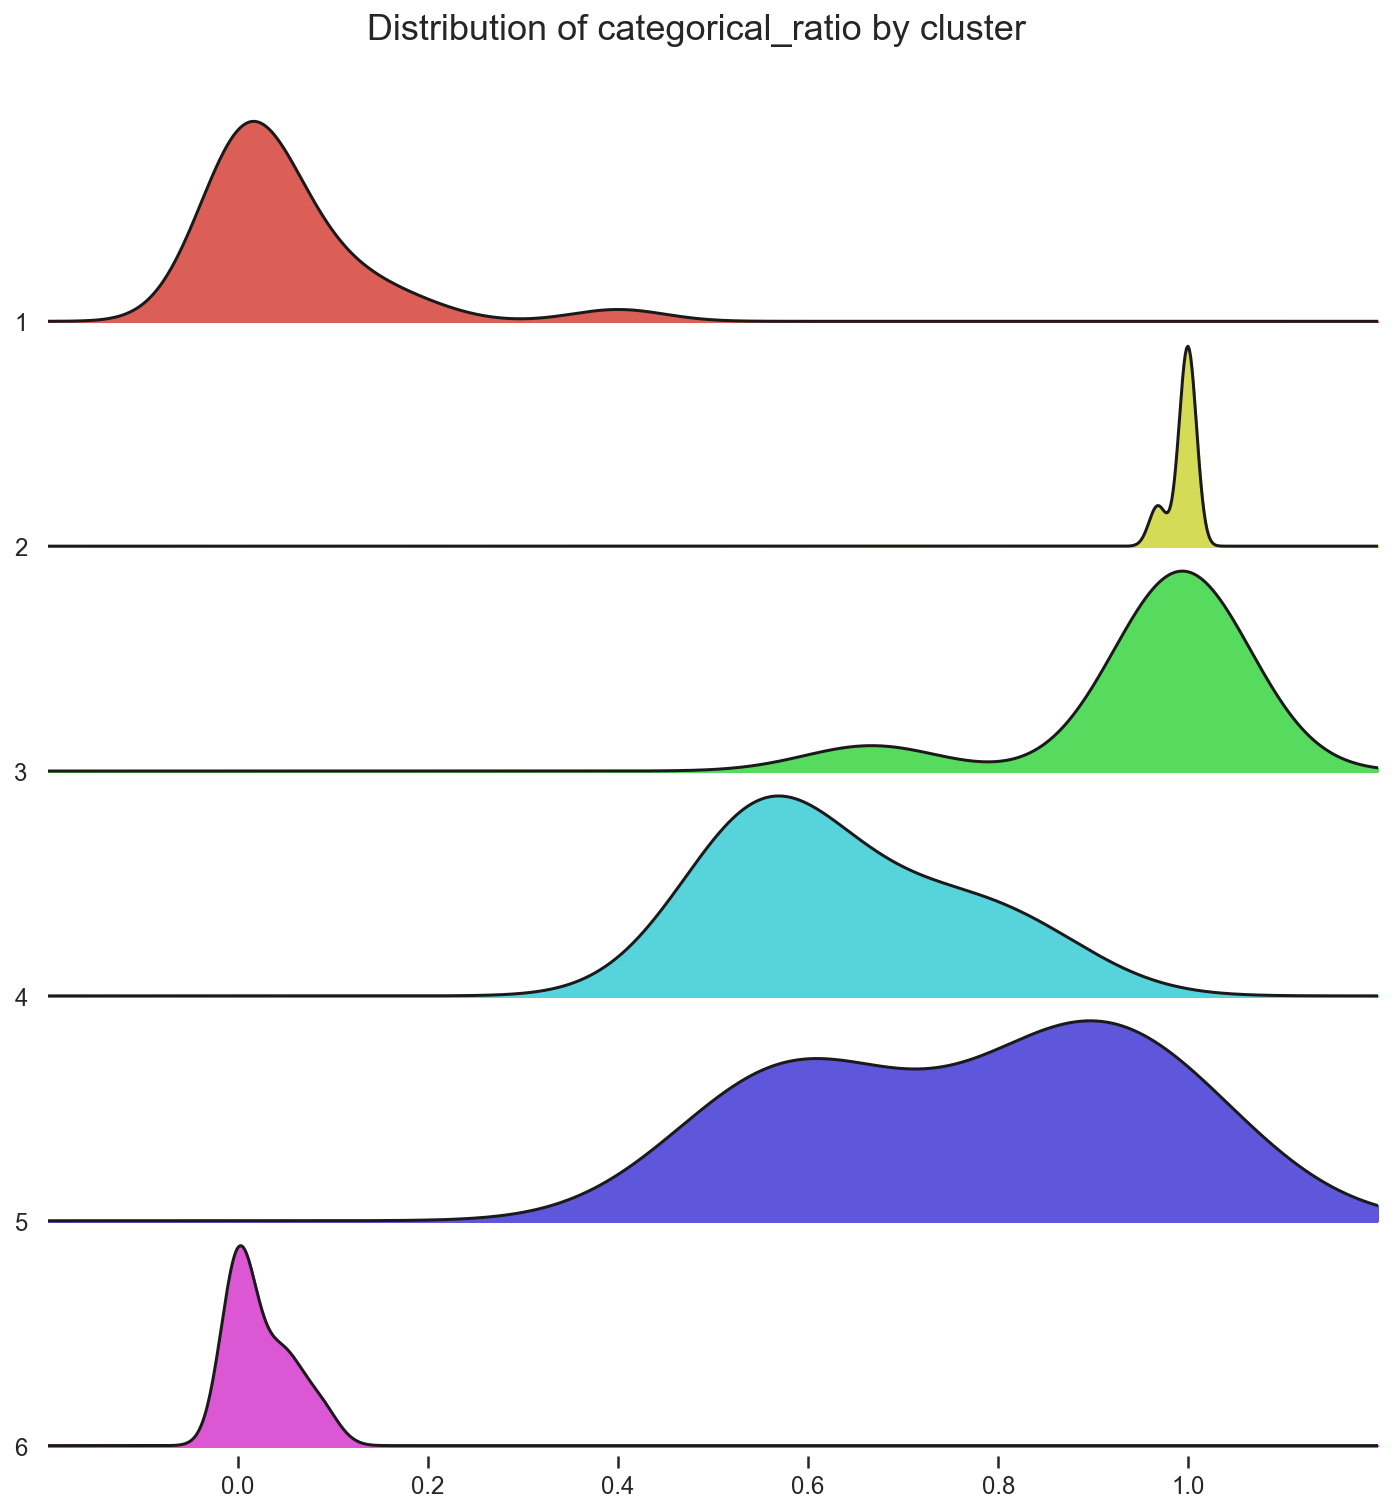
\includegraphics[width=.7\textwidth, height=.7\textwidth]{appendix_figures/joyplot_7.png}
    \caption{Ridgeline plot of \code{categorical\_ratio} }
\end{figure}
\begin{figure}[!ht]
    \centering
    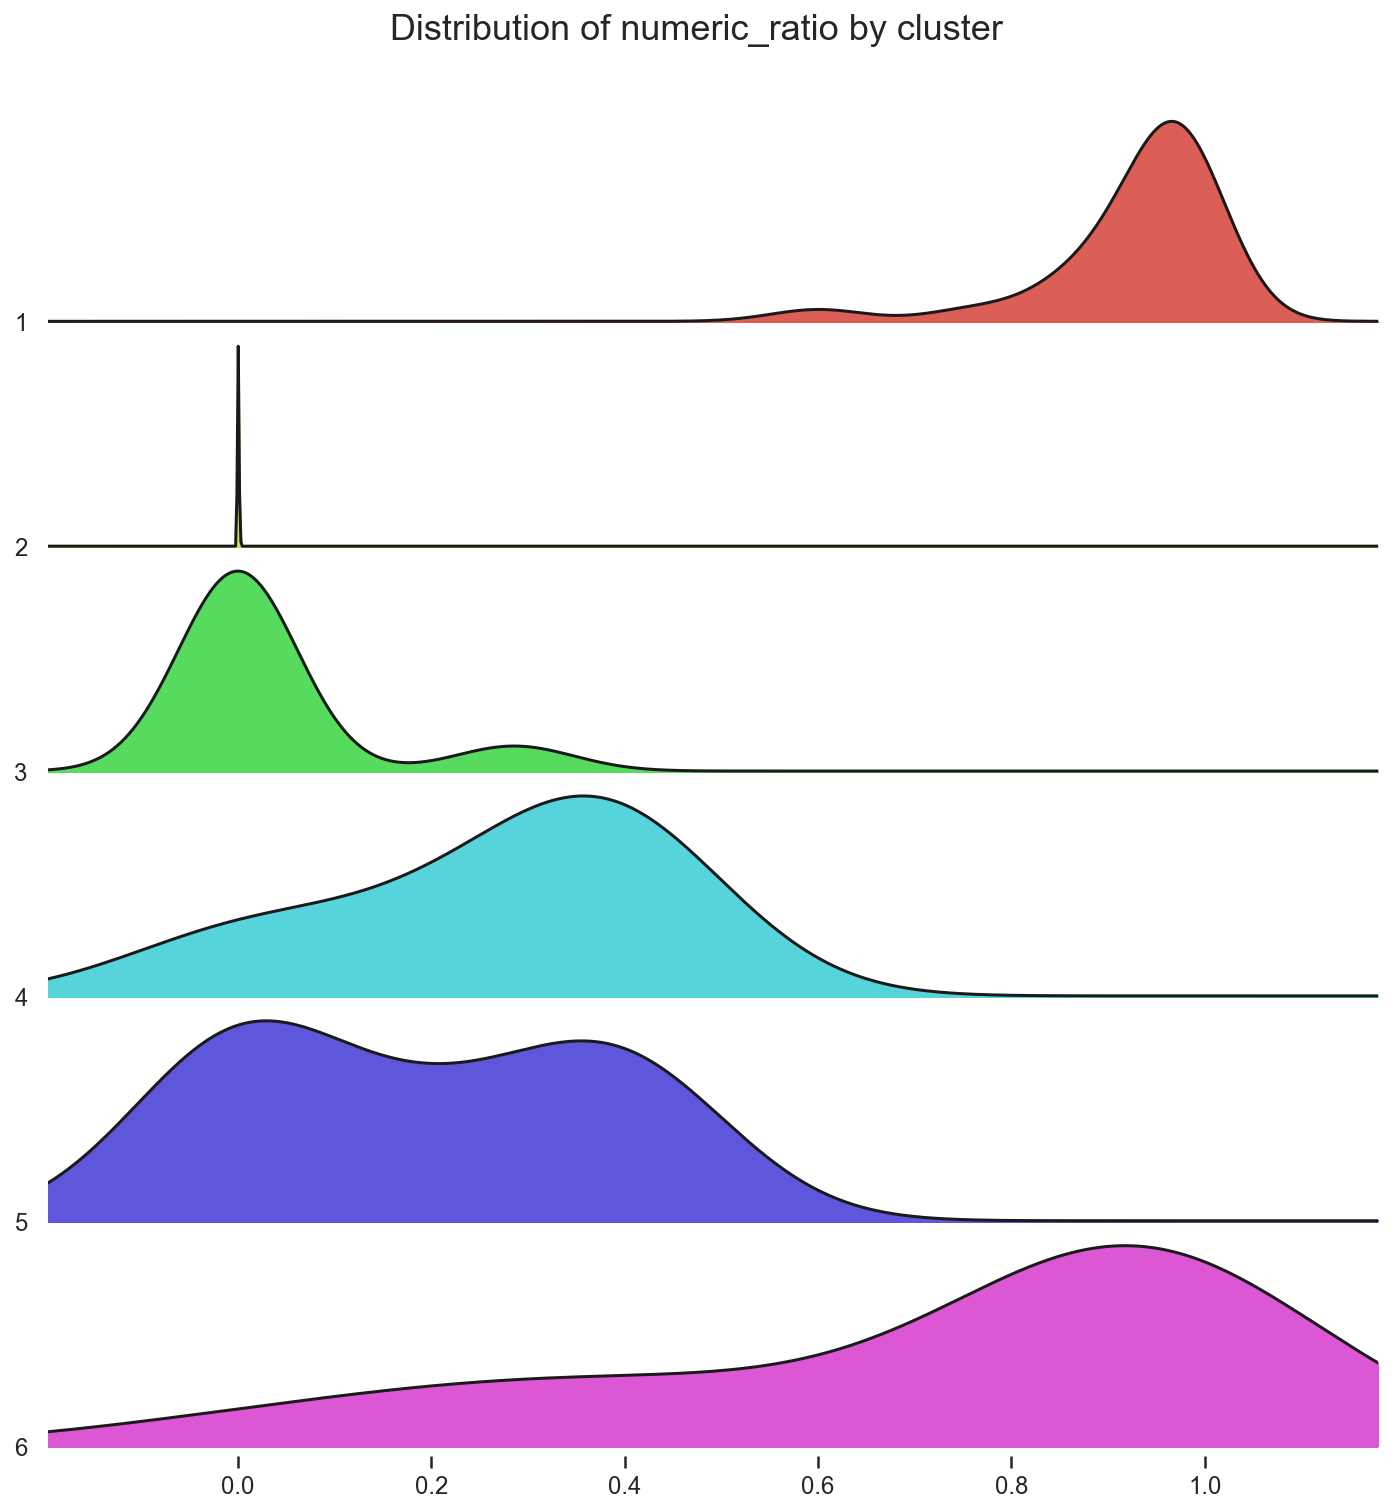
\includegraphics[width=.7\textwidth, height=.7\textwidth]{appendix_figures/joyplot_8.png}
    \caption{Ridgeline plot of \code{numeric\_ratio} }
\end{figure}
\begin{figure}[!ht]
    \centering
    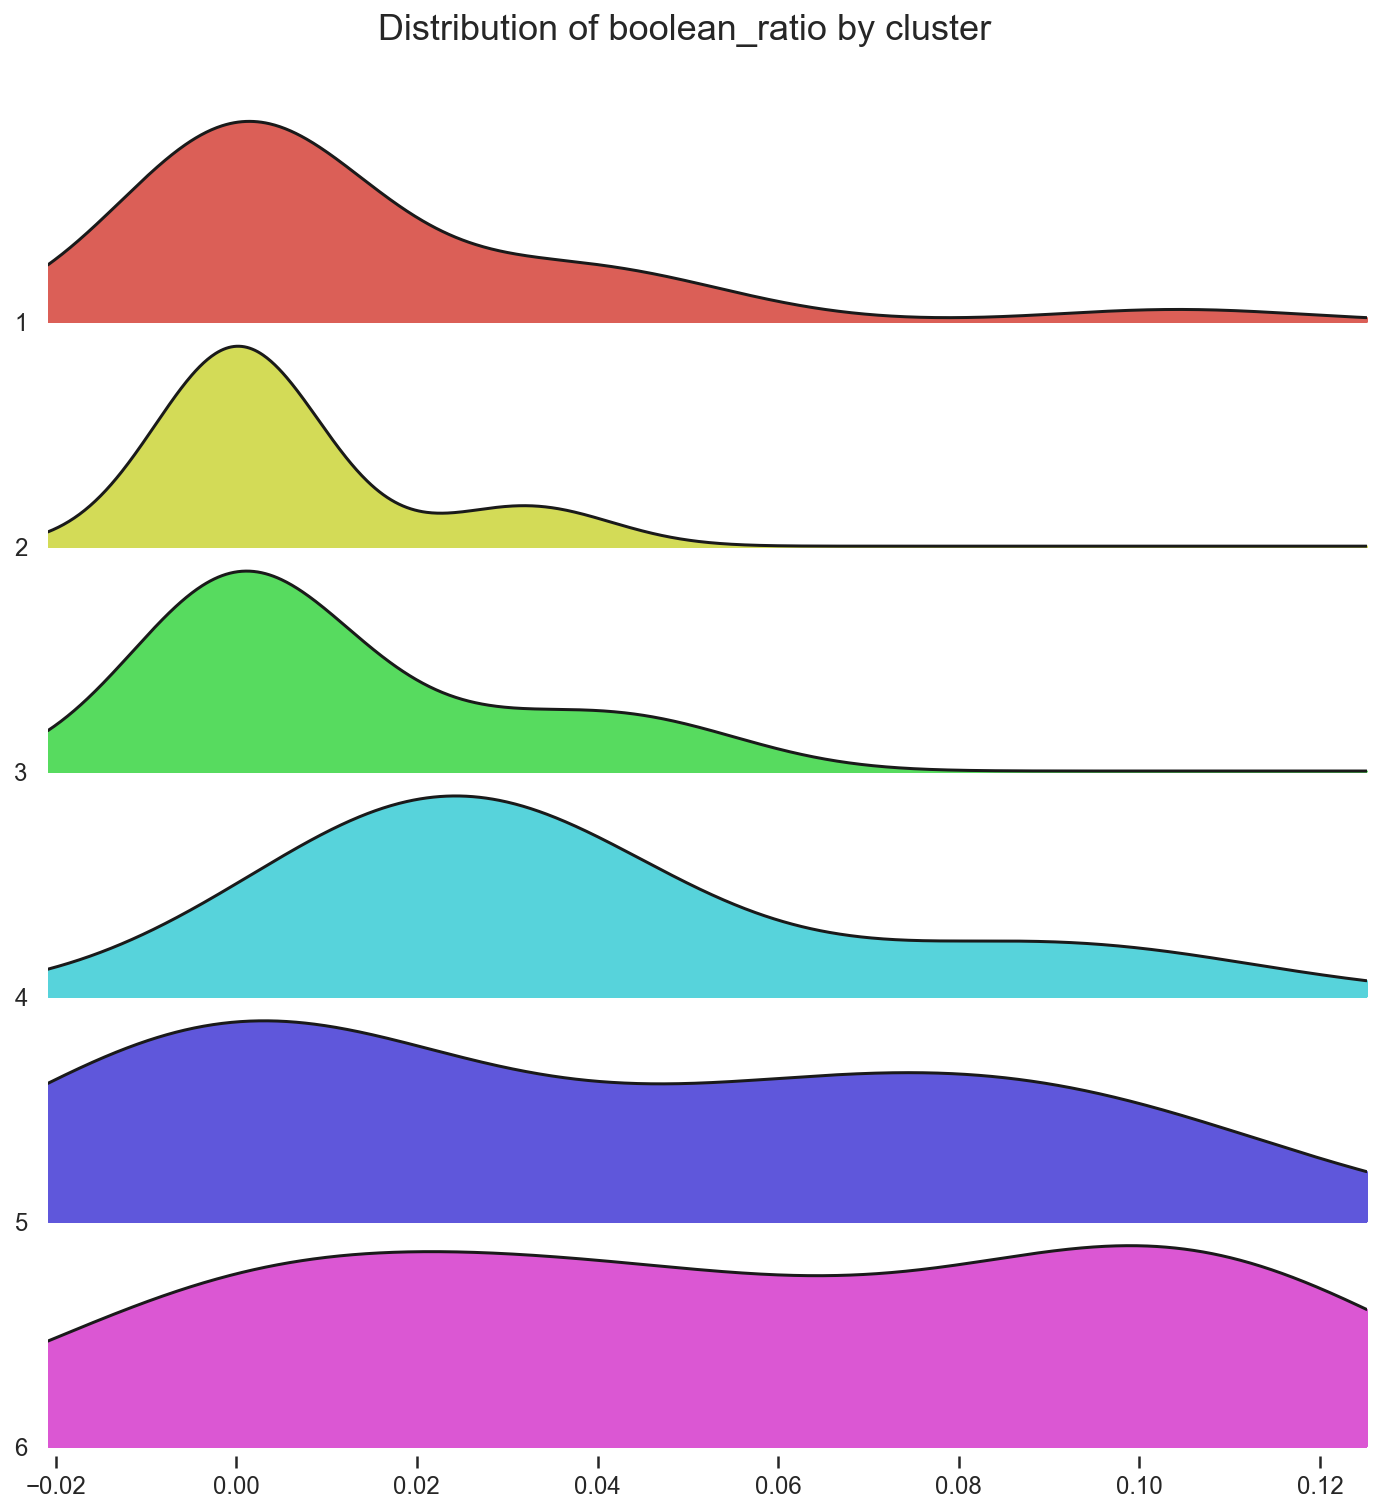
\includegraphics[width=.7\textwidth, height=.7\textwidth]{appendix_figures/joyplot_9.png}
    \caption{Ridgeline plot of \code{boolean\_ratio} }
\end{figure}